\documentclass[a4paper,11pt]{article}

%%%%%%%%%%%%%%%%%%%%%%%%%%%%%%%%%%%%%%%%%%%%%%%%%%%%%%%%%%%%%%%%%%%%%%%%%%%%%%%%%%%%%%%%%%%%%%%%%%%%%%%%%%%%%%%%%%%%%%%%%%%%%%
%%%%% output control / counter and macro hell
%%%%%%%%%%%%%%%%%%%%%%%%%%%%%%%%%%%%%%%%%%%%%%%%%%%%%%%%%%%%%%%%%%%%%%%%%%%%%%%%%%%%%%%%%%%%%%%%%%%%%%%%%%%%%%%%%%%%%%%%%%%%%%
\usepackage{ifthen}
\newcounter{include_sshots}
\setcounter{include_sshots}{0}

\newcommand{\sshots}[1]{\ifthenelse{\equal{\value{include_sshots}}{0}}{}{#1}}
\newcommand{\sshot}[1]{\sshots{\begin{center}\includegraphics[scale=.7]{#1}\end{center}}}
\newcommand{\sshotm}[1]{\sshots{\begin{center}\includegraphics[scale=.5]{#1}\end{center}}}


\newcounter{make_cover}
\setcounter{make_cover}{0}

\newcounter{ver_major}
\newcounter{ver_minor}


\newcounter{include_windows}
\setcounter{include_windows}{0}
\newcounter{include_mac}
\setcounter{include_mac}{0}
\newcounter{include_linux}
\setcounter{include_linux}{0}
\newcounter{include_all}
\setcounter{include_all}{0}
\newcounter{mac_or_lin}
\newcounter{mac_and_lin}


\newcommand{\maclin}{
  \ifthenelse{\equal{\value{mac_and_lin}}{0}}{\ifthenelse{\equal{\value{include_mac}}{0}}{\ifthenelse{\equal{\value{include_linux}}{0}}{}{Linux}}{Mac}}{Linux and Mac}}

\newcommand{\incwin}[1]{\ifthenelse{\equal{\value{include_windows}}{1}}{#1}{}}
\newcommand{\incmaclin}[1]{\ifthenelse{\equal{\value{mac_or_lin}}{1}}{#1}{}}
\newcommand{\incall}[1]{\ifthenelse{\equal{\value{include_all}}{1}}{#1}{}}

\newcommand{\printversion}{\arabic{ver_major}.\arabic{ver_minor}}

%%%%%%%%%%%%%%%%%%%%%%%%%%%%%%%%%%%%%%%%%%%%%%%%%%%%%%%%%%%%%%%%%%%%%%%%%%%%%%%%%%%%%%%%%%%%%%%%%%%%%%%%%%%%%%%%%%%%%%%%%%%%%%
%%%%% definitions
%%%%%%%%%%%%%%%%%%%%%%%%%%%%%%%%%%%%%%%%%%%%%%%%%%%%%%%%%%%%%%%%%%%%%%%%%%%%%%%%%%%%%%%%%%%%%%%%%%%%%%%%%%%%%%%%%%%%%%%%%%%%%%

\makeatletter
\newcommand\code{\bgroup\@makeother\_\@makeother\~\@makeother\$\@codex}
\def\@codex#1{{\normalfont\ttfamily\hyphenchar\font=-1 #1}\egroup}
\makeatother
%%\let\code=\texttt
\let\proglang=\textsf

\newcommand{\pkg}[1]{{\fontseries{b}\selectfont #1}}

\newcommand{\bX}{\boldsymbol{X}}
\newcommand{\bx}{\boldsymbol{x}}
\newcommand{\by}{\boldsymbol{y}}
\newcommand{\bbeta}{\boldsymbol{\beta}}
\newcommand{\bepsilon}{\boldsymbol{\epsilon}}


\newcommand{\ltwo}[1]{\left|\left| #1 \right|\right|_2}
\newcommand{\norm}[1]{\left|\left| #1 \right|\right|}


\newcommand\mnote[1]{\marginpar{\vspace*{-.8cm}#1}}

\newcommand\easy{\mnote{\LARGE\color{green} \textbf{Easy}}}
\newcommand\medium{\mnote{\LARGE\color{yellow2} \textbf{Medium}}}
\newcommand\hard{\mnote{\LARGE\color{red} \textbf{Hard}}}

%%%%%%%%%%%%%%%%%%%%%%%%%%%%%%%%%%%%%%%%%%%%%%%%%%%%%%%%%%%%%%%%%%%%%%%%%%%%%%%%%%%%%%%%%%%%%%%%%%%%%%%%%%%%%%%%%%%%%%%%%%%%%%
%%%%% paragraph spacing
%%%%%%%%%%%%%%%%%%%%%%%%%%%%%%%%%%%%%%%%%%%%%%%%%%%%%%%%%%%%%%%%%%%%%%%%%%%%%%%%%%%%%%%%%%%%%%%%%%%%%%%%%%%%%%%%%%%%%%%%%%%%%%
\usepackage{parskip}
\setlength{\parskip}{.3cm}

\usepackage[utf8]{inputenc}
\usepackage[margin=0.75in]{geometry}


%%%%%%%%%%%%%%%%%%%%%%%%%%%%%%%%%%%%%%%%%%%%%%%%%%%%%%%%%%%%%%%%%%%%%%%%%%%%%%%%%%%%%%%%%%%%%%%%%%%%%%%%%%%%%%%%%%%%%%%%%%%%%%
%%%%% colors
%%%%%%%%%%%%%%%%%%%%%%%%%%%%%%%%%%%%%%%%%%%%%%%%%%%%%%%%%%%%%%%%%%%%%%%%%%%%%%%%%%%%%%%%%%%%%%%%%%%%%%%%%%%%%%%%%%%%%%%%%%%%%%
\usepackage{xcolor}
\usepackage{color}

\definecolor{yellow2}{rgb}{1, .7, 0}

\definecolor{mygreen}{RGB}{0,150,0}

\definecolor{gray}{rgb}{.6,.6,.6}
\definecolor{dkgray}{rgb}{.3,.3,.3}
\definecolor{orange}{rgb}{1,0.5,0}
\definecolor{grayish}{rgb}{.9, .9, .9}

\definecolor{g11}{rgb}{0, 0, 1}
\definecolor{g12}{rgb}{0, .4, 1}
\definecolor{g13}{rgb}{0, .8, 1}

\definecolor{g21}{rgb}{0, .5, .3}
\definecolor{g22}{rgb}{.4, .5, .3}
\definecolor{g23}{rgb}{.8, .5, .3}

\definecolor{dkgreen}{rgb}{0,0.6,0}
\definecolor{mauve}{rgb}{0.58,0,0.82}

\definecolor{p0}{RGB}{150,0,0}
\definecolor{p1}{RGB}{0,150,0}
\definecolor{p2}{RGB}{0,0,150}
\definecolor{p3}{RGB}{150,75,0}


%%%%%%%%%%%%%%%%%%%%%%%%%%%%%%%%%%%%%%%%%%%%%%%%%%%%%%%%%%%%%%%%%%%%%%%%%%%%%%%%%%%%%%%%%%%%%%%%%%%%%%%%%%%%%%%%%%%%%%%%%%%%%%
%%%%% lstlisting
%%%%%%%%%%%%%%%%%%%%%%%%%%%%%%%%%%%%%%%%%%%%%%%%%%%%%%%%%%%%%%%%%%%%%%%%%%%%%%%%%%%%%%%%%%%%%%%%%%%%%%%%%%%%%%%%%%%%%%%%%%%%%%
\usepackage{listings}
\usepackage{ifpdf}

\lstdefinelanguage{sh}{basicstyle=\ttfamily\color{white}, backgroundcolor=\color{black}, breaklines=true} 

\ifpdf
\lstdefinelanguage{rr}{language=R, 
                      basicstyle=\ttfamily\color{black}, 
		      backgroundcolor=\color{grayish}, 
		      frame=single, 
		      breaklines=true, 
                      keywordstyle=\color{blue},
		      commentstyle=\color{dkgreen},
		      stringstyle=\color{mauve},
		      numbers=left,%none,
		      numberstyle=\tiny\color{dkgray},
		      stepnumber=1,       
		      numbersep=8pt,      
		      showspaces=false,      
		      showstringspaces=false,  
		      showtabs=false,     
		      rulecolor=\color{gray},   
		      tabsize=4,     
		      captionpos=t,
		      title=\lstname,
		      escapechar=?
% 		      escapeinside={(*@}{@*)},
% 		      escapebegin={\begin{lrbox}{0}\minipage[t]{.3\linewidth}\raggedleft\normalfont\itshape\small\leavevmode\color{black!70}\ignorespaces},
%                       escapeend={\endminipage\end{lrbox}\llap{\raisebox{0pt}[0pt][0pt]{\box0}\hspace{\comsep}}}
} 

\else

\lstdefinelanguage{rr}{basicstyle=\ttfamily\color{black}, 
		       backgroundcolor=\color{grayish}, 
		       frame=single, 
		       breaklines=true, 
		       tabsize=2
%                       keywordstyle=\color{blue},
% 		      commentstyle=\color{dkgreen},
% 		      stringstyle=\color{mauve}
} 

\fi


\lstnewenvironment{rr}{%
  \lstset{%
     language = R,%
      style    = default,%
    }%
 }{}





% \lstdefinelanguage{ft}{
%   language=[90]Fortran,
%   basicstyle=\ttfamily,
%                       keywordstyle=\color{blue},
% 		      commentstyle=\color{dkgreen},
%   morecomment=[l]{!\ }
% }



% \lstset{numbers=none,numberstyle=\footnotesize\ttfamily,
%         frame=single,frameround=tttt,language=R,
%         showspaces=false,showstringspaces=false,
%         breaklines=true,breakatwhitespace=true,
%         basicstyle=\small\ttfamily}
%\lstset{literate={<-}{{$\leftarrow$}}1}
% \makeatletter
% \let\Code\@undefined
% \let\CodeInput\@undefined
% \let\CodeOutput\@undefined
% \makeatother
% \lstnewenvironment{Command}[1][title=Shell Command]{\lstset{#1}}{}
% \lstnewenvironment{Code}[1][title=R Script]{\lstset{#1}}{}
% \lstnewenvironment{CodeOutput}[1][title=R Output]{\lstset{#1}}{}
% \lstnewenvironment{Error}[1][]{
%   \lstset{title=Error Message,basicstyle=\small\ttfamily}\color{Red}}{}
  

\makeatletter
\let\Code\@undefined
\let\CodeInput\@undefined
\let\CodeOutput\@undefined
\makeatother
\lstnewenvironment{Command}[1][]{\lstset{#1}}{}
\lstnewenvironment{Code}[1][]{\lstset{#1}}{}
\lstnewenvironment{CodeOutput}[1][]{\lstset{#1}}{}
\lstnewenvironment{Error}[1][]{
  \lstset{title=Error Message,basicstyle=\small\ttfamily}\color{Red}}{}
  
  
%%%%%%%%%%%%%%%%%%%%%%%%%%%%%%%%%%%%%%%%%%%%%%%%%%%%%%%%%%%%%%%%%%%%%%%%%%%%%%%%%%%%%%%%%%%%%%%%%%%%%%%%%%%%%%%%%%%%%%%%%%%%%%
%%%%% Chapter headings
%%%%%%%%%%%%%%%%%%%%%%%%%%%%%%%%%%%%%%%%%%%%%%%%%%%%%%%%%%%%%%%%%%%%%%%%%%%%%%%%%%%%%%%%%%%%%%%%%%%%%%%%%%%%%%%%%%%%%%%%%%%%%%
% \usepackage[Bjornstrup]{fncychap}
% \usepackage[Lenny]{fncychap}


%%%%%%%%%%%%%%%%%%%%%%%%%%%%%%%%%%%%%%%%%%%%%%%%%%%%%%%%%%%%%%%%%%%%%%%%%%%%%%%%%%%%%%%%%%%%%%%%%%%%%%%%%%%%%%%%%%%%%%%%%%%%%%
%%%%% Headers/footers
%%%%%%%%%%%%%%%%%%%%%%%%%%%%%%%%%%%%%%%%%%%%%%%%%%%%%%%%%%%%%%%%%%%%%%%%%%%%%%%%%%%%%%%%%%%%%%%%%%%%%%%%%%%%%%%%%%%%%%%%%%%%%%

\usepackage{lastpage}
\usepackage{fancyhdr}

\pagestyle{fancy}

\newcommand{\prebodyheadfoot}{
  \fancyhf{} % clear all header and footer fields
  \fancyfoot{}
  \renewcommand{\headrulewidth}{0pt}
  \renewcommand{\footrulewidth}{0pt}
  
  % redefinition of the plain style:
  \fancypagestyle{plain}{%
  \fancyhf{} % clear all header and footer fields
  \renewcommand{\headrulewidth}{0pt}
  \renewcommand{\footrulewidth}{0pt}}
}

\newcommand{\bodyheadfoot}{
  \fancyhf{} % clear all header and footer fields
%   \fancyhead[L]{\slshape \rightmark}
  \fancyhead[L]{\slshape \leftmark}
  \fancyhead[R]{ \thepage\ of\ \pageref{LastPage}}
  \fancyfoot[C]{\hrule Version \printversion}
  \renewcommand{\headrulewidth}{1pt}
  \renewcommand{\footrulewidth}{0pt}
  
  % redefinition of the plain style:
  \fancypagestyle{plain}{%
  \fancyhf{} % clear all header and footer fields
  \renewcommand{\headrulewidth}{0pt}
  \renewcommand{\footrulewidth}{0pt}}
}

%%%%%%%%%%%%%%%%%%%%%%%%%%%%%%%%%%%%%%%%%%%%%%%%%%%%%%%%%%%%%%%%%%%%%%%%%%%%%%%%%%%%%%%%%%%%%%%%%%%%%%%%%%%%%%%%%%%%%%%%%%%%%%
%%%%% Fancy toc originally from http://tex.stackexchange.com/questions/35825/pretty-table-of-contents?lq=1
%%%%%%%%%%%%%%%%%%%%%%%%%%%%%%%%%%%%%%%%%%%%%%%%%%%%%%%%%%%%%%%%%%%%%%%%%%%%%%%%%%%%%%%%%%%%%%%%%%%%%%%%%%%%%%%%%%%%%%%%%%%%%%
\usepackage{xcolor}
\usepackage{framed}
\usepackage{tikz}
\usepackage{titletoc}
\usepackage{etoolbox}
\usepackage{lmodern}


%%%%%%%%%%%%%%%%%%%%%%%%%%%%%%%%%%%%%%%%%%%%%%%%%%%%%%%%%%%%%%%%%%%%%%%%%%%%%%%%%%%%%%%%%%%%%%%%%%%%%%%%%%%%%%%%%%%%%%%%%%%%%%
%%%%% misc.
%%%%%%%%%%%%%%%%%%%%%%%%%%%%%%%%%%%%%%%%%%%%%%%%%%%%%%%%%%%%%%%%%%%%%%%%%%%%%%%%%%%%%%%%%%%%%%%%%%%%%%%%%%%%%%%%%%%%%%%%%%%%%%

% \usepackage{url}
\usepackage{amsmath}
\usepackage{amsthm}
\usepackage{amssymb}
% \usepackage{subfig}


\usepackage{hyperref}

\hypersetup{
    pdfnewwindow=true,    
    colorlinks=true,      
    linkcolor=blue,      
    citecolor=blue,      
    filecolor=magenta,   
    urlcolor=blue      
}

\usepackage[absolute]{textpos}


\input{.cover_ct} % control for whether the cover is included or not
\input{.pic_ct} % control for whether screenshots are included or not 
\input{.sec_ct} % control for which sections are included


%%% Document version
% Major
\setcounter{ver_major}{1}
% Minor
\setcounter{ver_minor}{0}



%%% for testing
% \setcounter{include_windows}{1}
% \setcounter{include_mac}{1}
% \setcounter{include_linux}{1}
% % 
% \setcounter{include_sshots}{1}
% \setcounter{make_cover}{0}



% counter voodoo
\ifthenelse{\equal{\value{include_mac}}{1} \OR \equal{\value{include_linux}}{1}}{\setcounter{mac_or_lin}{1}}{}
\ifthenelse{\equal{\value{include_mac}}{1} \AND \equal{\value{include_linux}}{1}}{\setcounter{mac_and_lin}{1}}{}
\ifthenelse{\equal{\value{include_mac}}{1} \AND \equal{\value{include_linux}}{1} \AND \equal{\value{include_windows}}{1}}{\setcounter{include_all}{1}}{}



\title{\Huge Setting Up a \proglang{pbdR} Environment\\[.3cm] 
  {\LARGE Installing MPI, \proglang{R}, and \proglang{pbdR}\\[.4cm]Version \printversion}}

\author{
\begin{minipage}{\textwidth}
\centering
%
\vspace{1cm}Prepared by the pbdR Core Team:\\[.8cm]
%
Drew Schmidt\\
{\small\emph{Remote Data Analysis and Visualization Center,\\
University of Tennessee, Knoxville}}\\[.4cm]
%%%
Wei-Chen Chen\\
{\small\emph{Computer Science and Mathematics Division, \\
Oak Ridge National Laboratory}}\\[.4cm]
%%%
Pragneskumar Patel\\
{\small\emph{Remote Data Analysis and Visualization Center,\\
University of Tennessee, Knoxville}}\\[.4cm]
%
George Ostrouchov\\
{\small\emph{Computer Science and Mathematics Division, \\
Oak Ridge National Laboratory}}
%%%
\end{minipage}
}


\begin{document}
% \ifpdf \else
% \Css{div.lstlisting{
%     font-family: monospace;
%     white-space: nowrap; margin-top:0.5em;
%     margin-bottom:0.5em;
%     color: black;
%     background-color: gray;
%   } 
%   div.verbatim{
%     font-family: monospace;
%     white-space: nowrap; margin-top:0.5em;
%     margin-bottom:0.5em;
%     color: white;
%     background-color: black;
%   }
% }
\ifpdf \else
\Css{div.lstlisting{font-family: monospace;
    white-space: nowrap; margin-top:0.5em;
    margin-bottom:0.5em;
    color: green ;
    background-color: black;}}

\Preamble{xhtml}
  \Configure{graphics*}  
         {pdf}  
         {\Needs{"convert \csname Gin@base\endcsname.pdf  
                               \csname Gin@base\endcsname.png"}%  
          \Picture[pict]{\csname Gin@base\endcsname.png}%  
         }  
\fi




\prebodyheadfoot

\ifthenelse{\equal{\value{make_cover}}{0}}{}{
  \begin{textblock*}{0mm}(-10.5mm,-8mm)
  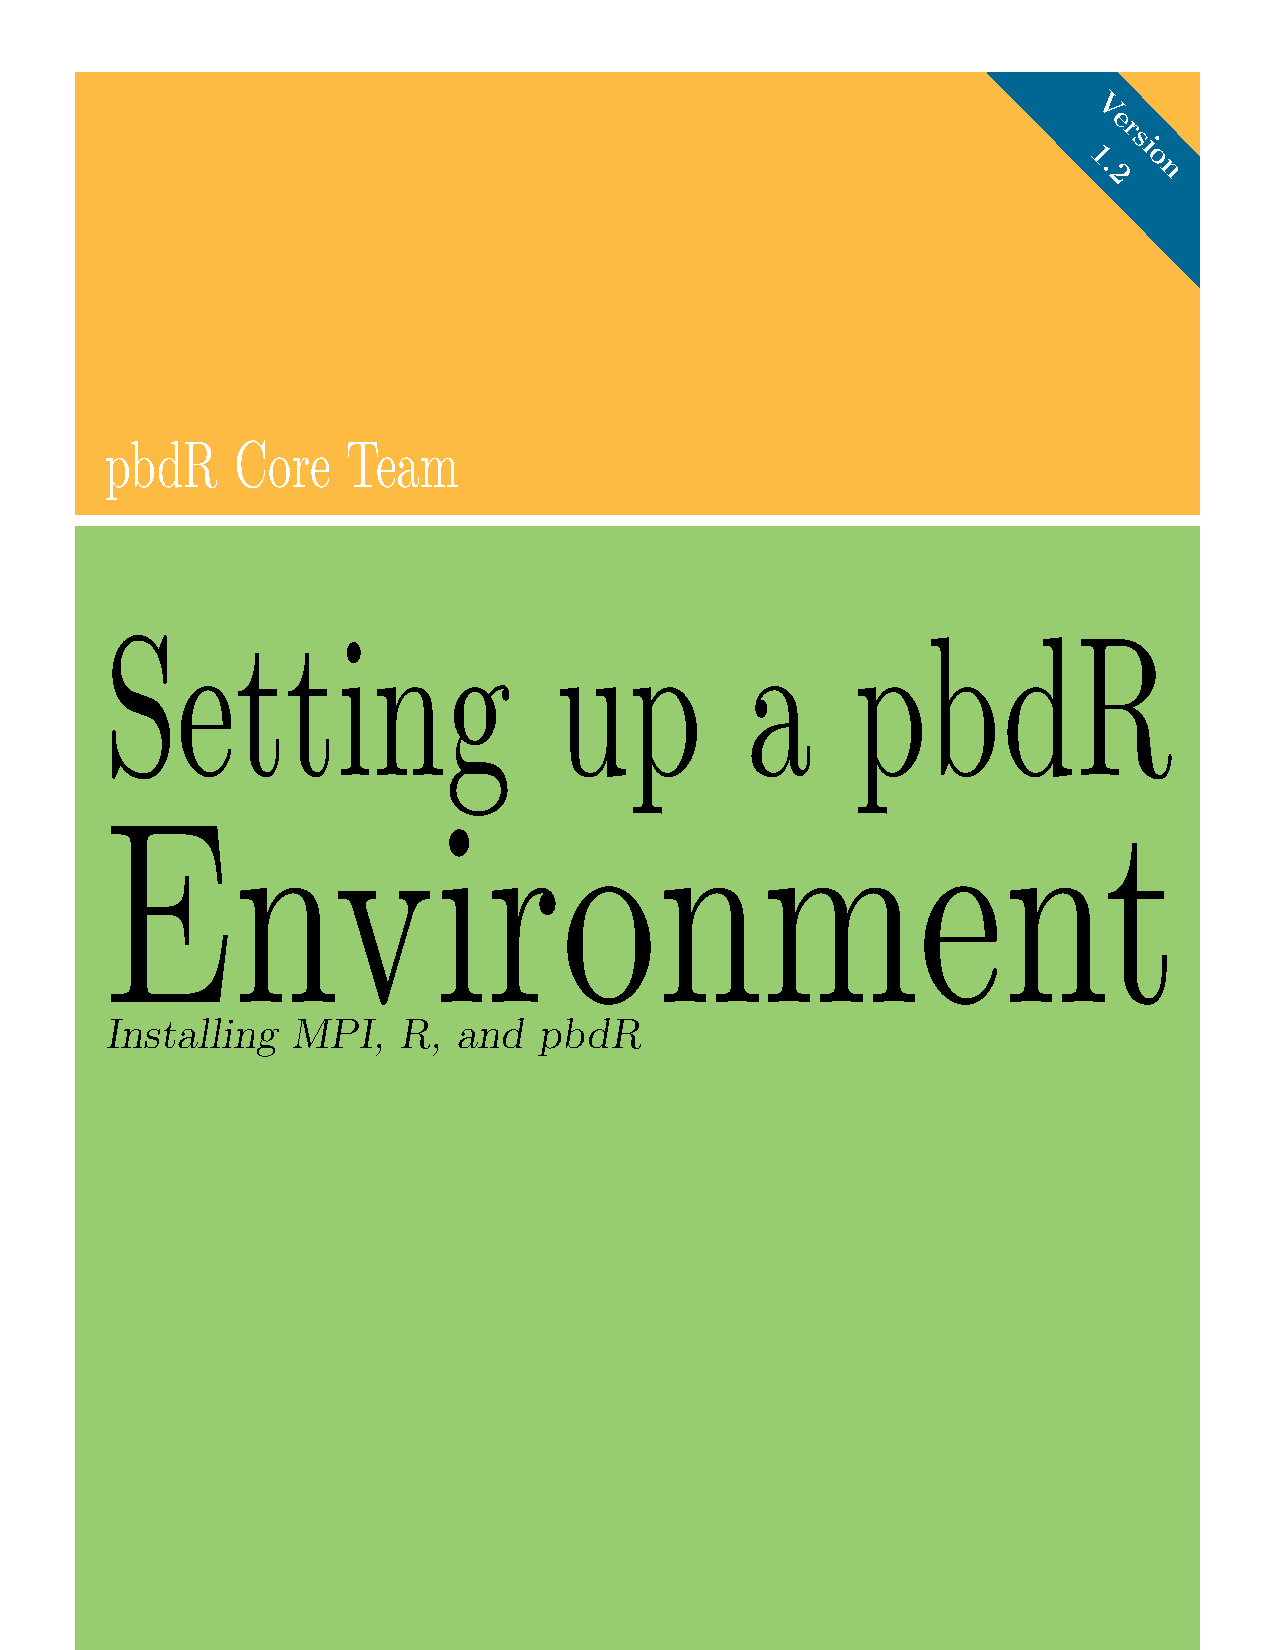
\includegraphics[scale=1.07]{./_all/cover/cover_2.pdf}
  \end{textblock*}
  \newpage\ \newpage
}


\date{}
\maketitle

%%%%%%%%%%%%%%%%%
\ \vfill

\copyright\ 2013 pbdR Core Team.  All rights reserved.

Permission is granted to make and distribute verbatim copies of this manual provided the copyright notice and this permission notice are preserved on all copies.

Permission is granted to copy and distribute modified versions of this manual under the conditions for verbatim copying, provided that the entire resulting derived work is distributed under the terms of a permission notice identical to this one.

Permission is granted to copy and distribute translations of this manual into another language, under the above conditions for modified versions, except that this permission notice may be stated in a translation approved by the pbdR Core Team. 

This publication was typeset using \LaTeX.  

%%%%%%%%%%%%%%%%%

\pagenumbering{roman}
\newpage
\fancyhf[C]{CONTENTS}
\fancyhf[R]{\thepage }
\fancyfoot{}
\tableofcontents

% ----------------------
% Body
% ----------------------

\newpage
\pagenumbering{arabic}
\setcounter{page}{1}
\pagestyle{fancy}

% Body header/footer style
\bodyheadfoot



\section{Quick Introduction}

In this guide, we will detail the necessary steps for how to set up a \proglang{pbdR} environment.  What follows in the remaining sections is a very lengthy list of installation instructions; however, most users should find the process fairly straight-forward, and may not need (or want) all of the details we will provide unless something goes wrong.  In any case, the short version for setting up a pbdR environment is to:
\begin{enumerate}
  \item install \proglang{R} \incwin{(and Rtools for Windows)}\label{enum:r}; see \url{http://cran.r-project.org/}
  \item install an MPI library\label{enum:mpi}; \url{http://www.open-mpi.org/}, or \url{http://www.mpich.org/} for Windows
  \item install the pbdR packages; see \url{http://r-pbd.org/}
\end{enumerate}

Items \ref{enum:r} and \ref{enum:mpi} are interchangeable, and so if you already have \proglang{R} \incwin{(and additionally Rtools for Windows)} and/or an MPI library installed, then merely skip this/these step(s); there is no need to reinstall anything.

\subsection{Installing R}
This should be fairly painless.  \proglang{R} has binary packages for every operating system you have heard of (and some you haven't), and the install should go fine.  Of course, since \proglang{R} is open source, you are free to compile it yourself, should have have reason or need to do so.  You can find both the source as well as binaries at the \proglang{R} project's main site: \url{http://cran.r-project.org/}.  

Additionally, you may wish to customize your \proglang{R} build by compiling from source.  For example, you may wish to link \proglang{R} with a high performance linear algebra library, such as MKL.  See the \emph{R Installation and Administration Manual} at \url{http://cran.r-project.org/doc/manuals/R-admin.html} for full details.  


\subsection{Installing MPI}
\incmaclin{For Linux and Mac users, we recommend installing OpenMPI, which is available from \url{http://www.open-mpi.org/} in both binary and source formats.}  \incwin{Windows users should install MPICH2, available from  \url{http://www.mpich.org/} .} 


\subsection{Installing pbdR Packages}
All released pbdR packages are available from \url{http://cran.r-project.org/} which is the Comprehensive \proglang{R} Archive Network (CRAN).  This is similar to the CPAN for \proglang{perl} or CTAN for \LaTeX, although with many improvements and benefits over its competitors.

It is also possible to link pbdR with high performance linear algebra libraries, such as MKL.
\begin{figure}[h]
\centering
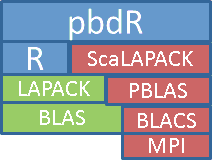
\includegraphics[scale=.7]{pics/libs.png}
\caption{pbdR Relationships to Libraries}\label{fig:pbd}
\end{figure}
Figure~\ref{fig:pbd} offers some insight into the package organization.  See the pbdSLAP vignette for more details.

\ifthenelse{\equal{\value{include_windows}}{0}}{}{
  \section{Windows}

Officially, the pbdR team does not support gaming consoles.  However, it is possible to install pbdR packages on Windows.

\subsection{R and Rtools}

The instructions and screenshots for this document are for version 2.15.1 of R, but later versions should be very similar, if not identical.






\subsubsection{R}


\begin{enumerate}
  \item Download R: \url{http://cran.r-project.org/bin/windows/base/} \label{enum:windl}
  \sshots{\begin{center}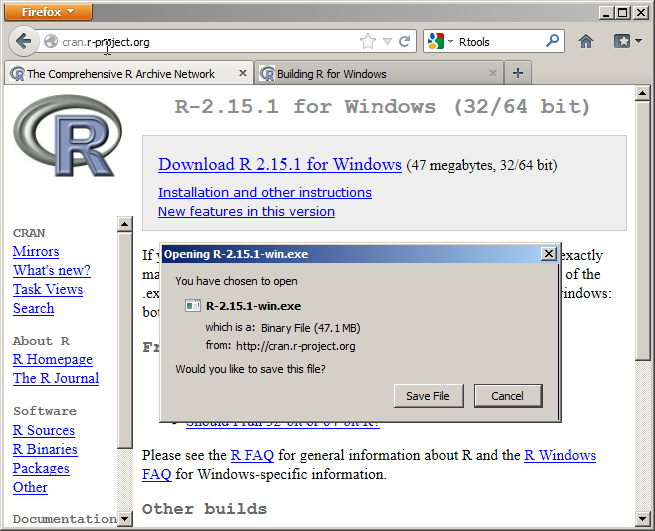
\includegraphics[scale=.5]{windows/pics/R_1.png}\end{center}}
  %
  \item Open the saved file from \ref{enum:windl} above to begin the installation.  At the first setup screen, click 'Next' to continue.
  \sshot{windows/pics/R_2.png}
  %
  \item When prompted with the license, click 'Next' to continue.
  \sshot{windows/pics/R_3.png}
  %
  \item When prompted for the location to install R, we strongly encourage you to use the default.  When you have made your decision, click 'Next'.
  \sshot{windows/pics/R_4.png}
    %
  \item When prompted with the components to install, you should select a 'User installation'.  Then click 'Next'.
  \sshot{windows/pics/R_5.png}
    %
  \item When prompted with the option to alter the startup options, we suggest selecting \code{No (accept defaults)}.  When you have made your decision, click 'Next'.
  \sshot{windows/pics/R_6.png}
    %
  \item When prompted with the start menu folder options, make your choice and then click 'Next'.
  \sshot{windows/pics/R_7.png}
    %
  \item When prompted with the additional tasks options, we suggest making sure that \code{Save version number in registry} and \code{Associate R with .RData files} are both \textbf{checked}.  When you have made your decisions, click 'Next'.
  \sshot{windows/pics/R_8.png}
  %
  \item To complete the R installation, select 'Finish'.
  \sshot{windows/pics/R_9.png}
  %
\end{enumerate}





\subsubsection{Rtools}

\begin{enumerate}
  \item Download Rtools: \url{http://cran.r-project.org/bin/windows/base/} \label{enum:rtoolsdl}
  \sshots{\begin{center}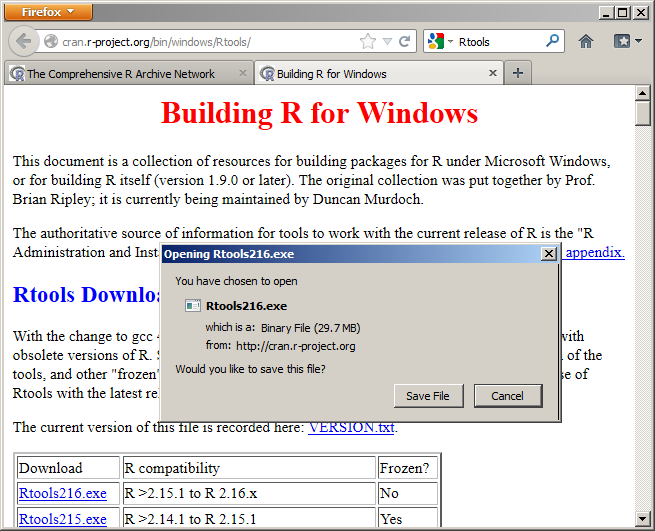
\includegraphics[scale=.5]{windows/pics/Rtools_1.png}\end{center}}
  %
  \item Open the saved file from \ref{enum:rtoolsdl} above to begin the installation.  At the first setup screen, click 'Next' to continue.
  \sshot{windows/pics/Rtools_2.png}
  %
  \item When prompted with the license, click 'Next' to continue.
  \sshot{windows/pics/Rtools_3.png}
  %
  \item When prompted for the location to install R, we strongly encourage you to use the default.  When you have made your decision, click 'Next'.
  \sshot{windows/pics/Rtools_4.png}
    %
  \item When prompted with the components to install, you should select a 'User installation'.  Then click 'Next'.
  \sshot{windows/pics/Rtools_5.png}
    %
  \item When prompted with the option to alter the startup options, we suggest selecting \code{No (accept defaults)}.  When you have made your decision, click 'Next'.
  \sshot{windows/pics/Rtools_6.png}
    %
  \item When prompted with the start menu folder options, make your choice and then click 'Next'.
  \sshot{windows/pics/Rtools_7.png}
    %
  \item To complete the Rtools installation, select 'Finish'.
  \sshot{windows/pics/Rtools_8.png}
  %
\end{enumerate}

}
\ifthenelse{\equal{\value{include_mac}}{0}}{}{
  \section{Mac OS X}

Before starting, make sure you have installed Apple's \href{https://developer.apple.com/xcode/}{XCode} package.  You can find this in the Mac App Store.  Additionally, during the course of installation, you may need to use the terminal once or twice.  You can launch it from Finder by navigating to the Applications folder; it should be called Terminal.app.  If you have never used the terminal before, you might consider skimming \href{http://guides.macrumors.com/Terminal}{this simple guide} on terminal basics.

If you are completely new to \proglang{R}, then you might consider reading (or at least skimming) this useful guide, \href{http://cran.r-project.org/bin/macosx/RMacOSX-FAQ.html}{R for Mac OS X FAQ}.  There is also the \href{http://cran.r-project.org/doc/FAQ/R-FAQ.html}{R FAQ} which may also be useful for those who know very little about \proglang{R}.  To learn more about programming with \proglang{R}, then you may find the \href{http://cran.us.r-project.org/doc/manuals/R-intro.html}{Introduction to R} guide useful.



\subsection{Installing R}

You can install \proglang{R} either from the binary package that CRAN builds (recommended) or from source.

\subsubsection{Installing from a Binary Package}

\begin{enumerate}
  \item First you should download \proglang{R} from the official distribution site: \url{http://cran.r-project.org/bin/macosx/} \label{enum:macdl}
  \sshots{\begin{center}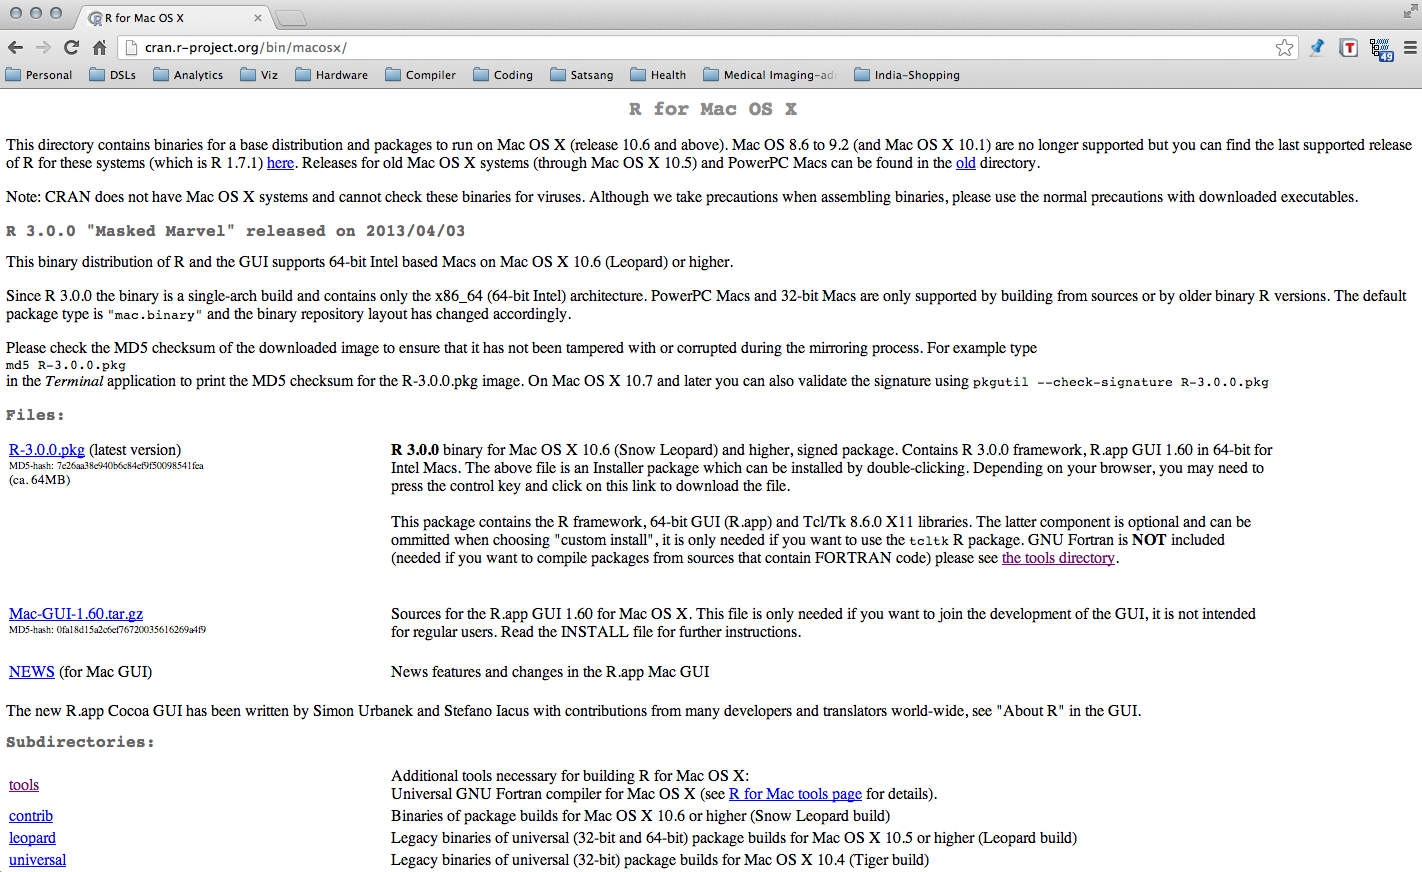
\includegraphics[scale=.3]{mac/pics/R_Mac_1.png}\end{center}}
  %
  Download the \proglang{R} dmg package for Mac OS X.  We recommend grabbing the latest version of \proglang{R} available.
  \sshots{\begin{center}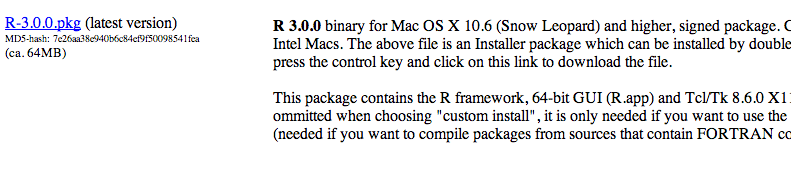
\includegraphics[scale=.7]{mac/pics/R_Mac_2_2.png}\end{center}}
  %
  \item Open the saved file from \ref{enum:macdl} above to begin the installation.  At the first setup screen, click 'Continue' to begin the installation process.
  \sshotm{mac/pics/R_Mac_3.png}
  %
  \item At the 'Read Me' section, read the important information and then click 'Continue'.
  \sshotm{mac/pics/R_Mac_4.png}
    %
  \item When prompted with the software license agreement, you must click 'Agree' to proceed.  \proglang{R} is distributed under a free, ``copyleft'' license (GPL v3).  You can read the license by clicking 'Read License'.  Once you agree to the terms, click 'Agree'.
  \sshotm{mac/pics/R_Mac_5.png}
    %
  \item From the 'Installation Type' section, we recommend you use the defaults.  However, you may change the install location by selecting 'Change Install Location\dots'.  Once you have made your choice, click 'Install'.
  \sshotm{mac/pics/R_Mac_6.png}
    %
  \item Next, you will be prompted for your computer's name and password.  Enter the appropriate information and click 'Install Software' to begin the installation process.
  \sshotm{mac/pics/R_Mac_7.png}
  %
  \item Once the installation process begins, wait a few moments for the packages to validate and install.
  \sshotm{mac/pics/R_Mac_8.png}
  %
  \sshotm{mac/pics/R_Mac_9.png}
  %
  \sshotm{mac/pics/R_Mac_10.png}
  %
  \sshotm{mac/pics/R_Mac_11.png}
  %
  \item Once the installation completes successfully, click 'Close' to finish the installation process.
  \sshotm{mac/pics/R_Mac_12.png}
  %
\end{enumerate}

Out of the box, you can run an interactive \proglang{R} session in two separate ways:  from the ``gui'' and from a terminal.  To launch the \proglang{R} ``gui'', simply go to your Applications folder in Finder and double-click \code{R.app}.
  \sshots{\begin{center}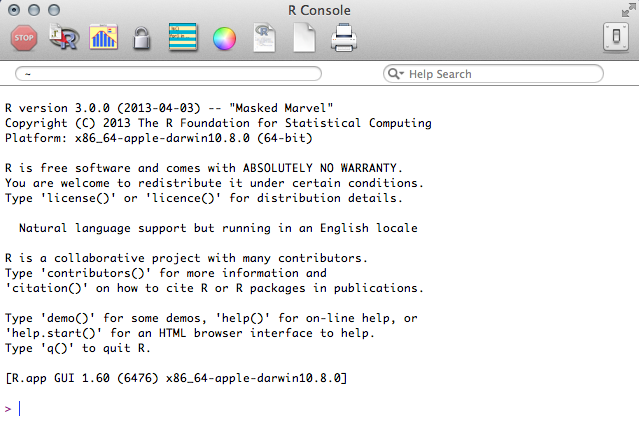
\includegraphics[scale=.8]{mac/pics/R_Mac_13.png}\end{center}}

Once \proglang{R} is finished installing, you need to install the  \href{http://cran.r-project.org/web/packages/rlecuyer/index.html}{\pkg{rlecuyer}} package.  To install it from an interactive \proglang{R} session, simply start an \proglang{R} session and issue the command
\begin{lstlisting}[language=rr]
install.packages("rlecuyer")
\end{lstlisting}





\subsubsection{Compiling from Source}

You can find \proglang{R} sources from \url{http://cran.r-project.org/sources.html}

Start by opening a terminal and navigate to the folder containing the \proglang{R} source package you just downloaded.  You can extract the archive by executing, for example
\begin{lstlisting}[language=sh]
tar zxvf R-3.0.0.tar.gz
\end{lstlisting}

From here, generally it should be enough to simply execute
\begin{lstlisting}[language=sh]
./configure && make && make install
\end{lstlisting}
without problems.









\subsection{Installing MPI}

You have several options for installing OpenMPI on a Mac.  You can install from \href{https://www.macports.org/}{MacPorts}, which is a relatively simple way to manage compiling/installing of many packages (such as OpenMPI).  You can also compile from source.

Before beginning, make sure you have some ``downtime'' allotted, as the compilation will take upwards of a few hours for some machines.

\subsubsection{Installing from a MacPorts}

Arguably the easiest way to install OpenMPI for a Mac (that I'm aware of) is using \href{https://www.macports.org/}{MacPorts}, which is not unlike some source repositories for Linux.  You can find information about installing MacPorts from \href{https://www.macports.org/install.php}{MacPorts installation page}, maintained by the MacPorts project.

Once you have MacPorts installed, you can install openmpi from a terminal by issuing the command:
\begin{lstlisting}[language=sh]
sudo port install openmpi
\end{lstlisting}





\subsubsection{Compiling from Source}

If you want to install OpenMPI from source (I don't really recommend this unless you think you have a good reason to), then the sources are available \href{http://www.open-mpi.org/software/ompi/v1.6/}{here}.





\subsection{Installing pbdR Packages}
Installing pbdR should go smoothly.  The simplest way to install the packages is from an \proglang{R} terminal, which will manage dependencies for you much like the Mac App store.


\subsubsection{Installing from CRAN}
This is perhaps the simplest way to proceed, as \proglang{R} will handle any package dependency resolution for you.  Simply start an \proglang{R} session (from the terminal\footnote{Do \emph{not} use the gui.  See section~\ref{sec:porblam} for details}, type \code{R} then press enter) and issue the command:
\begin{lstlisting}[language=rr]
install.packages(<package>)
\end{lstlisting}
So for example, to install \pkg{pbdMPI}, you might execute:
\begin{lstlisting}[language=rr]
install.packages(pbdMPI)
\end{lstlisting}


\subsubsection{Installing from the Shell}
If you have downloaded a pbdR (or other \proglang{R}) package, then installing from the shell simply amounts to issuing the command:
\begin{lstlisting}[language=sh]
R CMD INSTALL <package>
\end{lstlisting}
So for example, to install \pkg{pbdMPI}, you might execute:
\begin{lstlisting}[language=sh]
R CMD INSTALL pbdMPI_0.1-6.tar.gz
\end{lstlisting}


\subsubsection{Installing from Github}
CRAN policy is such that updates to packages can not be made too frequently.  For this reason, the development versions of our packages will have bugfixes and new features much more quickly than CRAN versions.  

The easiest way to install from github is using Hadley Wichkam's \pkg{devtools} package (which can be installed via \code{install.packages(devtools)}).  Assuming you have this package installed, then from an \proglang{R} session, to install a pbdR package you would issue one of the following:

\begin{lstlisting}[language=rr]
install_github(repo="pbdMPI", username="RBigData")
install_github(repo="pbdSLAP", username="RBigData")
install_github(repo="pbdNCDF4", username="RBigData")
install_github(repo="pbdBASE", username="RBigData")
install_github(repo="pbdDMAT", username="RBigData")
install_github(repo="pbdDEMO", username="RBigData")
\end{lstlisting}

You can also install \emph{really} new package builds, which will be very current in terms of features, but also bugs (or even complete package breakage).  If you're sure you want these packages, then you can install them as follows:

\begin{lstlisting}[language=rr]
# dev repo 1
install_github(repo="pbdMPI", username="snoweye")
install_github(repo="pbdSLAP", username="snoweye")
install_github(repo="pbdNCDF4", username="snoweye")
# dev repo 2
install_github(repo="pbdBASE", username="wrathematics")
install_github(repo="pbdDMAT", username="wrathematics")
install_github(repo="pbdDEMO", username="wrathematics")
\end{lstlisting}

}
\ifthenelse{\equal{\value{include_linux}}{0}}{}{
  \section{Linux and FreeBSD}

Before starting, you may need root access to your machine.  Also, you will need to know how to do some simple things via the terminal.  If you're using a standard Linux desktop, you probably have a terminal launcher in your applications menu somewhere.  If you're using some kind of weirdo tiling thing from 1990, then I assume you know what you're doing.  Additionally, if you are inexperienced with using the terminal, you should consider skimming \href{http://community.linuxmint.com/tutorial/view/100}{this short introduction}.

On Linux, unless you have a specific reason not to (in which case, most of this document is probably unnecessary for you), we recommend that you install \proglang{R} and MPI through your distribution's package repository (especially MPI).  This will make the installation process \emph{much} simpler, and generally ``just works''.

If instructions for your favorite distribution are not listed below, we would be happy to incorporate submissions/corrections.

Finally, if you are completely new to \proglang{R}, then you might consider reading the \href{http://cran.r-project.org/doc/FAQ/R-FAQ.html}{R FAQ}.  To learn more about programming with \proglang{R}, then you may find the \href{http://cran.us.r-project.org/doc/manuals/R-intro.html}{Introduction to R} guide useful.






\subsection{Installing R}

You can install \proglang{R} either from your package repo (recommended) or from source.

\subsubsection{Installing from a Package Repository}

If your distribution is Debian-derived, including Debian, Ubuntu, and Mint:
\begin{lstlisting}[language=sh]
apt-get install r-base-dev
\end{lstlisting}

\vspace{.4cm}
If your distribution is ``Redhat-ish'', including Redhat, Fedora, and CentOS:
\begin{lstlisting}[language=sh]
yum install R-devel
\end{lstlisting}

\vspace{.4cm}
If your distribution is OpenSUSE:
\begin{lstlisting}[language=sh]
zypper install R-patched-devel
\end{lstlisting}

\vspace{.4cm}
If you are using FreeBSD:
\begin{lstlisting}[language=sh]
cd /usr/ports/math/R && make install clean
\end{lstlisting}



\subsubsection{Compiling from Source}

You can find \proglang{R} sources from \url{http://cran.r-project.org/sources.html}

Start by opening a terminal and navigate to the folder containing the \proglang{R} source package you just downloaded.  You can extract the archive by executing, for example
\begin{lstlisting}[language=sh]
tar zxvf R-3.0.0.tar.gz
\end{lstlisting}

From here, generally it should be enough to simply execute
\begin{lstlisting}[language=sh]
./configure && make && make install
\end{lstlisting}
without problems.









\subsection{Installing MPI}

You can install \proglang{R} either from your package repo (recommended) or from source.

\subsubsection{Installing from a Package Repository}

For these systems, we recommend using OpenMPI.  To install OpenMPI

If your distribution is Debian-derived, including Debian, Ubuntu, and Mint:
\begin{lstlisting}[language=sh]
apt-get install openmpi-bin libopenmpi-dev
\end{lstlisting}

\vspace{.4cm}
If your distribution is ``Redhat-ish'', including Fedora and CentOS:
\begin{lstlisting}[language=sh]
yum install openmpi openmpi-devel
\end{lstlisting}

\vspace{.4cm}
If your distribution is OpenSUSE:
\begin{lstlisting}[language=sh]
zypper install openmpi-devel lam-devel
\end{lstlisting}

\vspace{.4cm}
If you are using FreeBSD:
\begin{lstlisting}[language=sh]
cd /usr/ports/net/openmpi && make install clean
\end{lstlisting}



\subsubsection{Compiling from Source}

If you want to install OpenMPI from source (I don't really recommend this unless you think you have a good reason to), then the sources are available \href{http://www.open-mpi.org/software/ompi/v1.6/}{here}.









\subsection{Installing pbdR Packages}
Installing pbdR should go smoothly.  The simplest way to install the packages is from an \proglang{R} terminal, which will manage dependencies for you much like your distro's package manager.  Additionally, our packages are available in the Fedora repositories.


\subsubsection{Installing from CRAN}
This is perhaps the simplest way to proceed, as \proglang{R} will handle any package dependency resolution for you.  Simply start an \proglang{R} session (from the terminal, type \code{R} then press enter) and issue the command:
\begin{lstlisting}[language=rr]
install.packages(<package>)
\end{lstlisting}
So for example, to install \pkg{pbdMPI}, you might execute:
\begin{lstlisting}[language=rr]
install.packages(pbdMPI)
\end{lstlisting}


\subsubsection{Installing from the Shell}
If you have downloaded a pbdR (or other \proglang{R}) package, then installing from the shell simply amounts to issuing the command:
\begin{lstlisting}[language=sh]
R CMD INSTALL <package>
\end{lstlisting}
So for example, to install \pkg{pbdMPI}, you might execute:
\begin{lstlisting}[language=sh]
R CMD INSTALL pbdMPI_0.1-6.tar.gz
\end{lstlisting}


\subsubsection{Installing from Github}
CRAN policy is such that updates to packages can not be made too frequently.  For this reason, the development versions of our packages will have bugfixes and new features much more quickly than CRAN versions.  

The easiest way to install from github is using Hadley Wichkam's \pkg{devtools} package (which can be installed via \code{install.packages(devtools)}).  Assuming you have this package installed, then from an \proglang{R} session, to install a pbdR package you would issue one of the following:

\begin{lstlisting}[language=rr]
library(devtools)

install_github(repo="pbdMPI", username="RBigData")
install_github(repo="pbdSLAP", username="RBigData")
install_github(repo="pbdNCDF4", username="RBigData")
install_github(repo="pbdNCDF4", username="RBigData")
install_github(repo="pbdBASE", username="RBigData")
install_github(repo="pbdDMAT", username="RBigData")
install_github(repo="pbdDEMO", username="RBigData")
\end{lstlisting}

You can also install \emph{really} new package builds, which will be very current in terms of features, but also bugs (or even complete package breakage).  If you're sure you want these packages, then you can install them as follows:

\begin{lstlisting}[language=rr]
# dev repo 1
install_github(repo="pbdMPI", username="snoweye")
install_github(repo="pbdSLAP", username="snoweye")
install_github(repo="pbdNCDF4", username="snoweye")
# dev repo 2
install_github(repo="SEXPtools", username="wrathematics")
install_github(repo="pbdBASE", username="wrathematics")
install_github(repo="pbdDMAT", username="wrathematics")
install_github(repo="pbdDEMO", username="wrathematics")
\end{lstlisting}

}

\section{Running pbdR Scripts}
This information is covered in \emph{much} more detail in the pbdDEMO vignette, and should not be considered a substitute.  However, 

\begin{itemize}
  \item pbdR codes are written in Single Program/Multiple Data style
  \item pbdR codes are executed in batch
\end{itemize}



\begin{lstlisting}[language=rr]
library(pbdMPI, quiet = TRUE)
init()

x <- comm.rank()

comm.print(x, all.rank = TRUE)

finalize()
\end{lstlisting}


\ifnum\value{mac_or_lin}=1
On \maclin, you should execute the command:
\begin{lstlisting}[language=sh]
mpirun -np 2 Rscript my_script.r
\end{lstlisting}
\fi

\ifnum\value{include_windows}=1
On Windows, you should execute the command:
\begin{lstlisting}[language=sh]
mpiexec.exe -np 2 Rscript my_script.r
\end{lstlisting}
\fi



\section{Installation Problems}

During the course of installation, you may run into unrecoverable issues.  The pbdR team does not support MPI libraries or R core, so if you have problems during that portion of the installation phase, we probably can not directly help you.  However, there are still many great resources at your disposal, maintained by those individual projects.

\subsection{R and MPI}

If you have problems installing or customizing R, see the \emph{R Installation and Administration Manual} at \url{http://cran.r-project.org/doc/manuals/R-admin.html} for help.

If you are having trouble installing an MPI library, you should see that library's official documentation.  For OpenMPI, see \url{http://www.open-mpi.org/community/help/} and for MPICH, see \url{http://www.mpich.org/documentation/guides/} .

For the remainder, we will be addressing installation issues with pbdR packages.

\subsection{pbdR}

This is a quick list of potential problems you could encounter when installing pbdR packages.  For additional troubleshooting or installation options, each package has a vignette which may offer additional useful information.

\begin{itemize}
  \item \textbf{When compiling pbdMPI from source}, you may be required to pass a configure argument at compile time.  So for example, if you have OpenMPI installed and were installing from the command line, then you would issue the command:
\begin{Code}
R CMD INSTALL pbdMPI_0.1-6.tar.gz \
        --configure-args='--with-Rmpi-type=OPENMPI'
\end{Code}
  or if installing from R:
  \begin{lstlisting}[language=rr]
install.packages("pbdMPI", configure.args='--with-Rmpi-type=OPENMPI')
\end{lstlisting}

  \item \textbf{If you are installing on a cluster} where you must install on the login node which can not load the packages, then pass the install option \code{--no-test-load}.    So for example, if installing from the command line, then you would issue the command:
\begin{Code}
R CMD INSTALL pbdMPI_0.1-6.tar.gz --no-test-load
\end{Code}
  or if installing from R:
  \begin{lstlisting}[language=rr]
install.packages("pbdMPI", INSTALL_opts='--no-test-load')
\end{lstlisting}
  
\end{itemize}



\end{document}
